%\section{EC-Cuts}
\subsection{Electromagnetic Calorimeter Cuts}    %  nwTgtEcCt = NewTgtECcuts(..) in ~/LinkedFiles/evS\subsection{Electromagnetic Calorimeter Cuts}    %  nwTgtEcCt = NewTgtECcuts(..) in ~/LinkedFiles/evSelectionCutsAllinOne.h
\label{ecCuts}

The EC cuts consist of two %three
different cuts applied together. One of these is on the sampling fraction i.e. the fraction of the energy deposited in the calorimeter, and the other is on the energy fraction deposited in the inner part of the calorimeter. % and the last is based on the correlation between the inner and outer energies recorded by the calorimeter.

\begin{comment}
%Inside NewTgtECcuts  we have the following with Q2 dependent values for sfCt (Using same width cut on the left as that for CLAS data
%    to ensure same fraction of data)
bool NewTgtECcuts(int DataOrSim,int Eb_index, float pp, float ei, float eo, float et, float beta, int Q2bin) 
{
  double sfCt=0.2, sfCut=0.2; if(Q2bin<15) sfCut=0.15;
  double sigmaTimes=(MeanSfClas[Q2bin]-sfCut)/SigmaSfClas[Q2bin]; //Distance of sfCut(==0.2 or 0.15 etc) from mean in units of sigma
  if(DataOrSim==1)
    {
      sfCt=sfCut; 
    }
  else if(DataOrSim==0)
    {
      sfCt=MeanSfSim[Q2bin] - SigmaSfSim[Q2bin]*sigmaTimes; //Using the same width cut on the left as that for CLAS data to ensure same fraction of data 
    }
  //See *.gif & *.txt files with name starting with ecCuts_sfOneD_Eb2 & ecCuts_eiOneD_Eb2 in http://wwwold.jlab.org/Hall-B//secure/eg4/adhikari/Analysis/SimStuffs/CutsPlots/ (Sim data made with VzD32, Vz=-100.93 & NewVzCuts(..) above.
  if( et/pp>sfCt    &&    ei>0.06    &&   (eo/pp >= -(0.20/0.11)*ei/pp + 0.20)) return true; else return false;
}
\end{comment}


\subsubsection{Cuts on EC sampling fraction}
%\textbf{\textcolor{red}{Comment: Show plots from one or two Q2 bins and list all other cuts in a table (may go to Appendix)}}
While moving through the EC, charged pions are minimum ionizing particles in the momentum range detectable by CLAS. On the other hand, each electron deposits its total energy $E_{tot}$ in the EC\footnote{Because some of the deposited energy is in the lead part of the EC rather than the scintillator, only a fraction of the electron energy is detected in the EC.} %\footnote{Due to occasional mismatching with momentum information from DC during the reconstruction process, $E_{tot}$ is not always calculated to be the sum of the energies deposited in the inner and outer parts of EC. Therefore, in our analysis, we calculate $E_{in}$ + $E_{out}$ and if this sum turns out to be larger than $E_{tot}$, then we choose the sum as the true value of $E_{tot}$.} 
by %undergoing/
producing electromagnetic showers. %($E_{tot} \approx p$ for electrons that have high energies). %which is proportional to its momentum p. 
Therefore, the sampling fraction $E_{tot}/p$ should be independent of the momentum for electrons (in reality there is a slight dependence). 

\begin{figure}[H] %ht, htpb (p - float, b = bottom, h=? t = top)
%\leavevmode 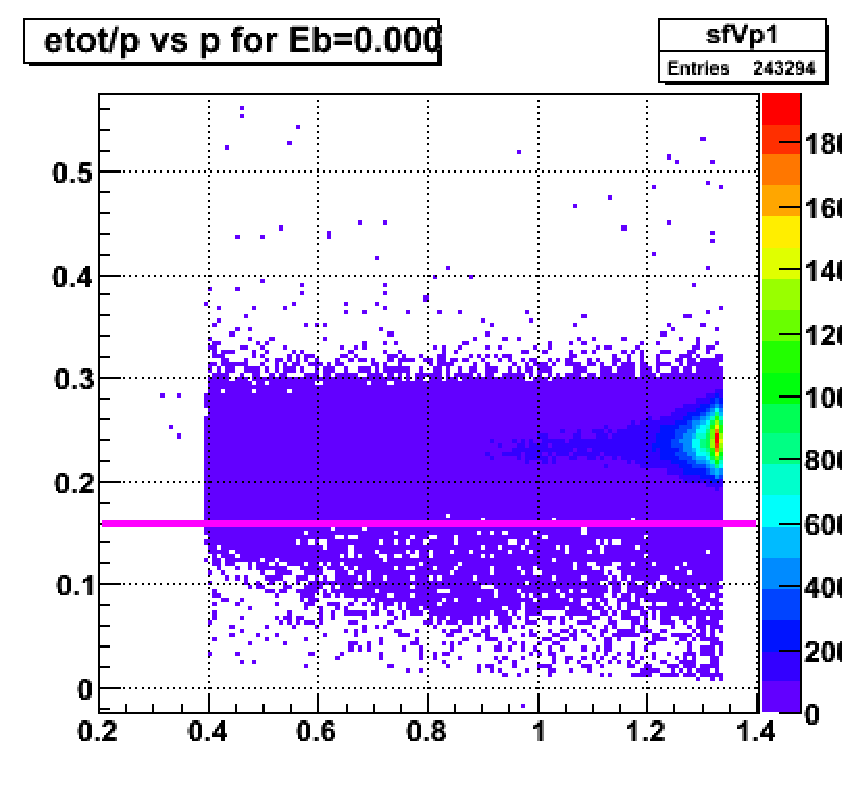
\includegraphics[width=1.0\textwidth]{chap4simul/FigConv/stdECcutsSfvP_Eb1.eps}  %0.6 is the fraction of the real image width????
\centering
%\leavevmode 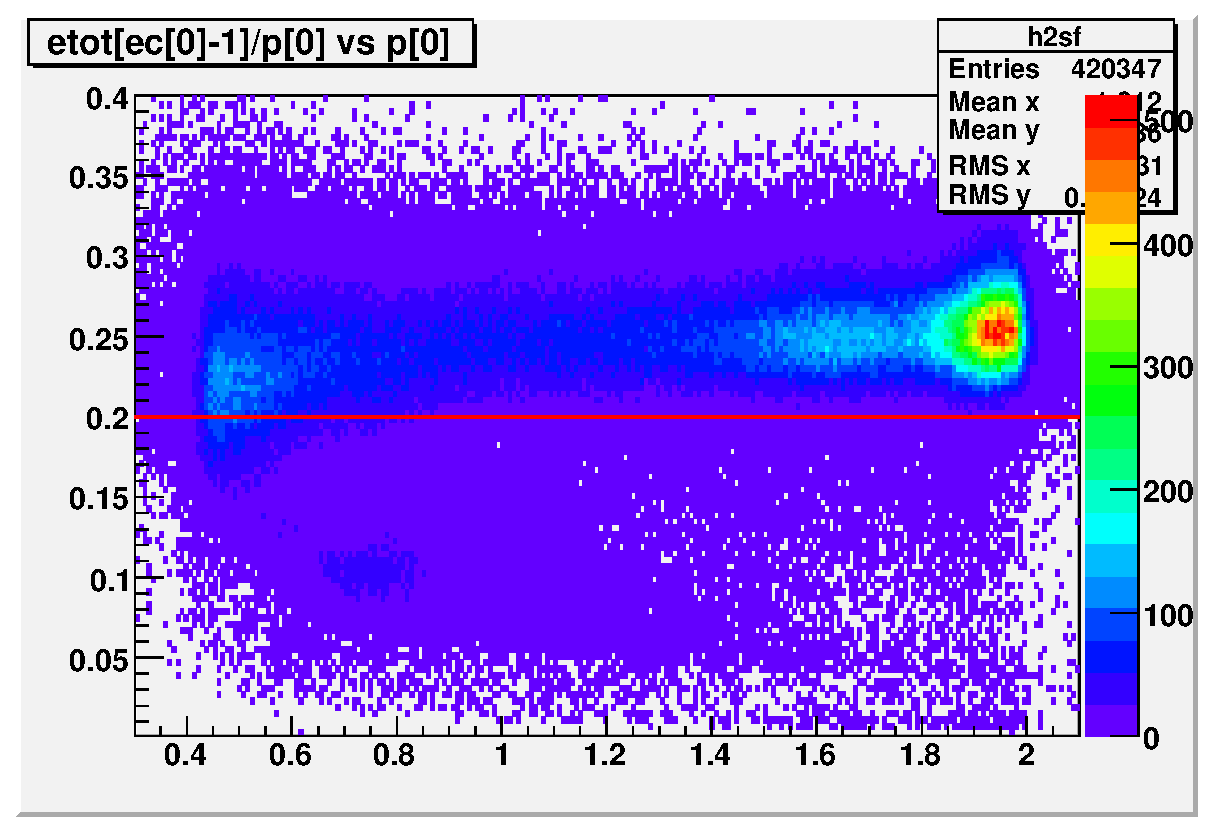
\includegraphics[width=1.0\textwidth]{figuresEG4/FigCuts/ecCuts_sfVp2D_Eb2allEv.eps}  %2.0 GeV data
\leavevmode 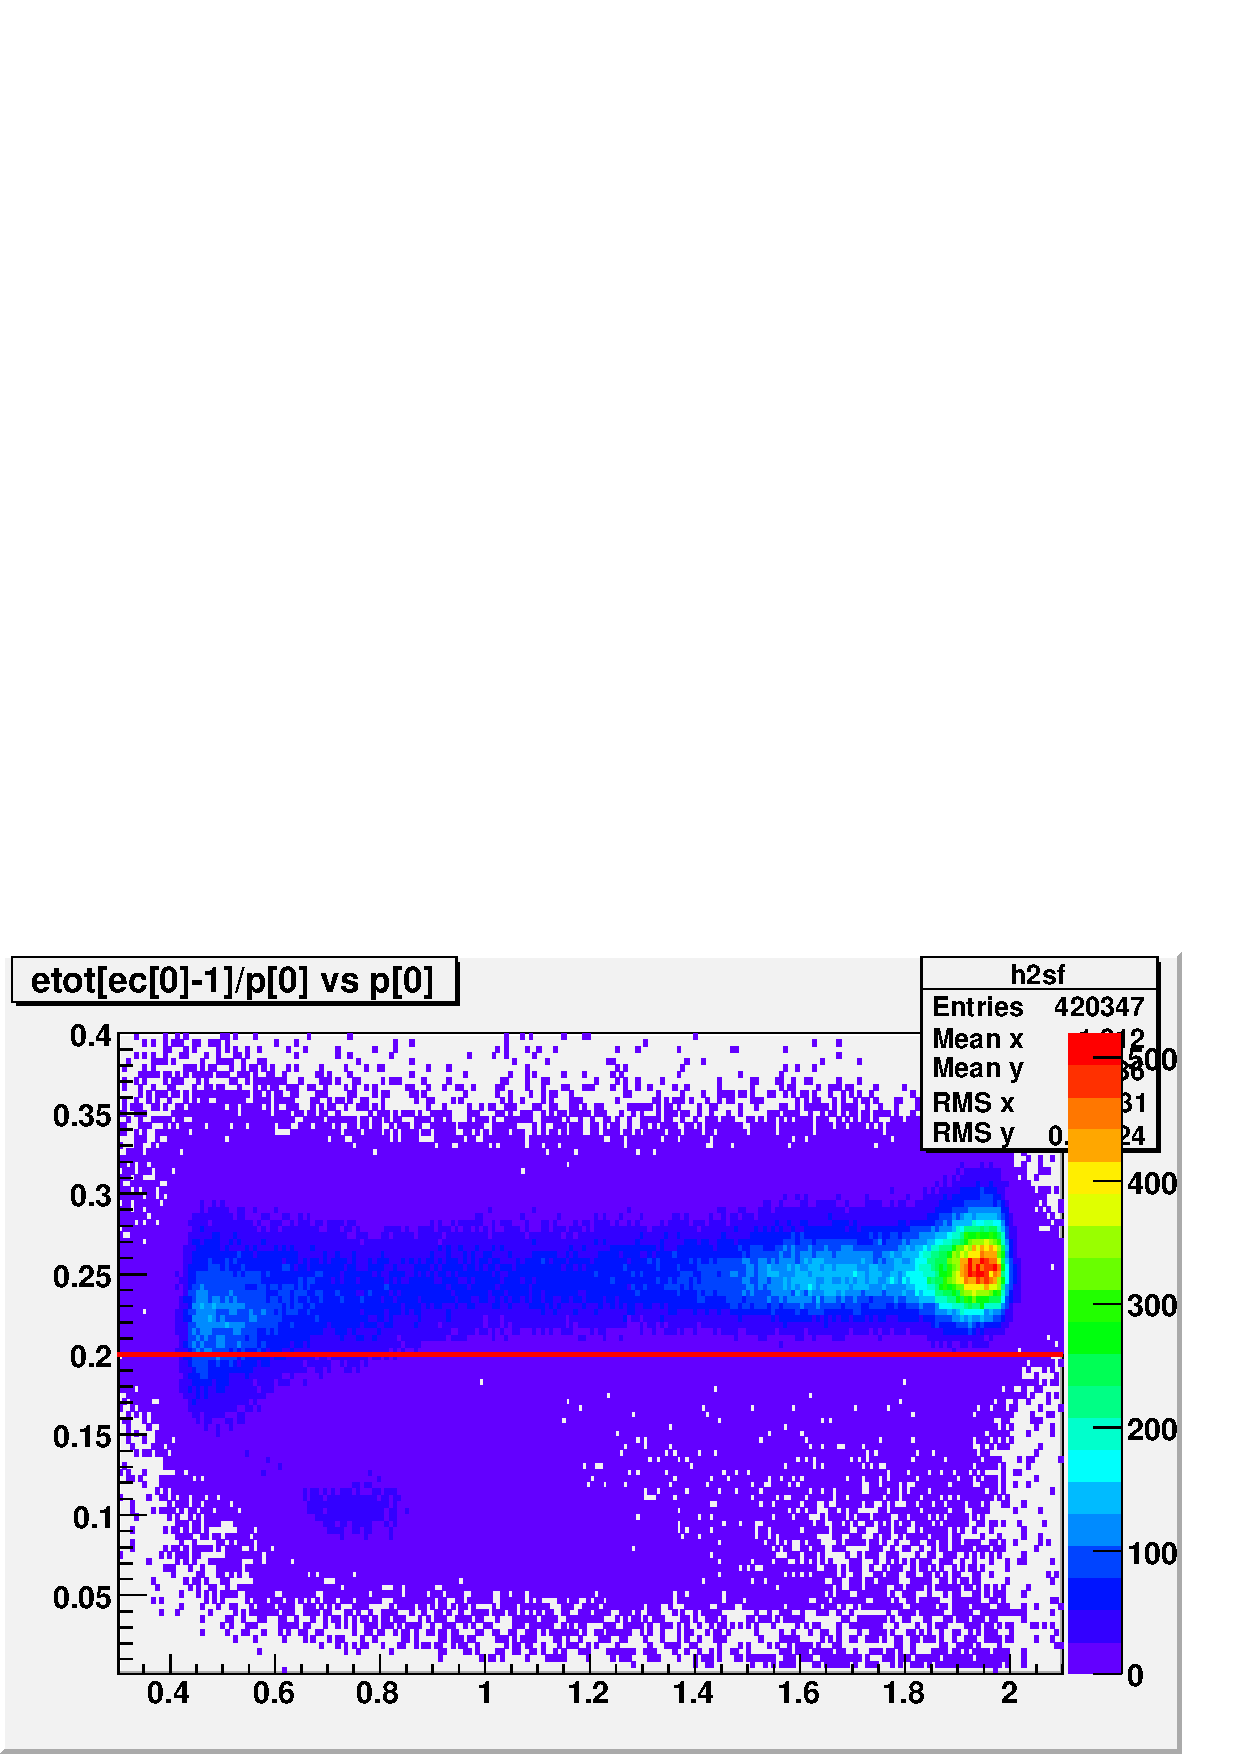
\includegraphics[width=0.8\textwidth]{figuresEG4/FigCuts/ecCuts_sfVp2D_Eb2allEv.png}  %2.0 GeV data
\caption[EC sampling fraction cut (2.0 GeV)]{An example of the cut on the EC sampling fraction (2.0 GeV data). The plots shows the distribution of the sampling fraction (in Y-axis) plotted against the particle momentum (in X-axis). The brighter stripe above about 0.2 in the energy fraction are due to the electrons whereas those below are the pions.
 %\textcolor{red}{SEK: Y-label (Sampling fraction); arrow/or texts indicating pions and electrons. This figure is not very clear - could you use logarithmic z scale? \\ GED: What are the exes? Units? What do we see here?}
}
\label{ecSf}
\end{figure}


%In case of EC in the CLAS, 
For the EC in CLAS, the electron sampling fraction ($etot/p$) is about 0.25 and pions give signals that are mostly below 0.2 (see Fig. \ref{ecSf} or others that follow). Therefore, a lower cut of $etot/p > 0.2$ is usually chosen to reject most of the pions without significantly losing good electrons. However, in %the case of 
our low beam energy experiment, %with its low beam energy, %being relatively smaller, 
few pions are produced and the electron peaks are cleaner in lower kinematic bins as can be seen in the low \qsqs bins of Fig. \ref{ecSfExp6}. Therefore, %in order to have fewer good electrons rejected, 
a \qsqs bin dependent cut of $etot/p > (\mu - 3\sigma)$ was chosen, where $\mu$ and $\sigma$ are the Gaussian fit parameters representing the mean and standard deviation of the distribution in the corresponding \qsqs bin. 
The choice of $3 \sigma$ was decided by looking at the sampling fraction distributions in each of the \qsqs bins and making sure that no pion signal was observed in any of the bins.


On simulated data also, a corresponding $3 \sigma$ cut was applied by first repeating the exact same procedure to get the corresponding values of $\mu$ and $\sigma$ from the simulated data. Using same-$\sigma$ cuts %(i.e. the same relative distance from the electron peaks) 
in corresponding \qsqs bins of both experimental and simulated data ensures that we had the same fraction of data in corresponding bins from both experimental and simulated sides. 



\begin{figure}[H]%[htp] %ht, htpb (p - float, b = bottom, h=? t = top)
\centering
%\leavevmode 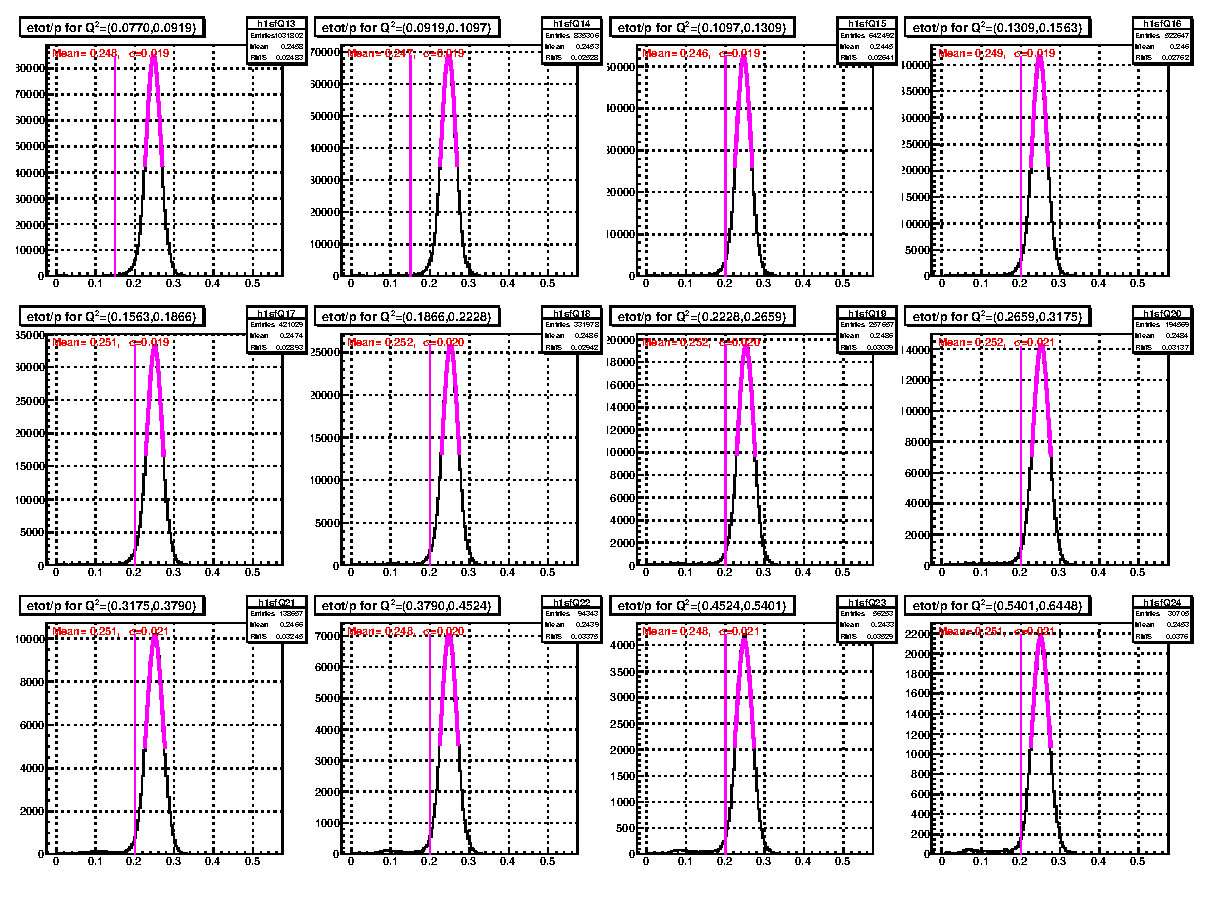
\includegraphics[width=1.0\textwidth]{chap4simul/FigCuts/ecCuts_sfOneD_Eb2_4Th.eps}  %0.6 is the fraction of the real image width????
%\leavevmode 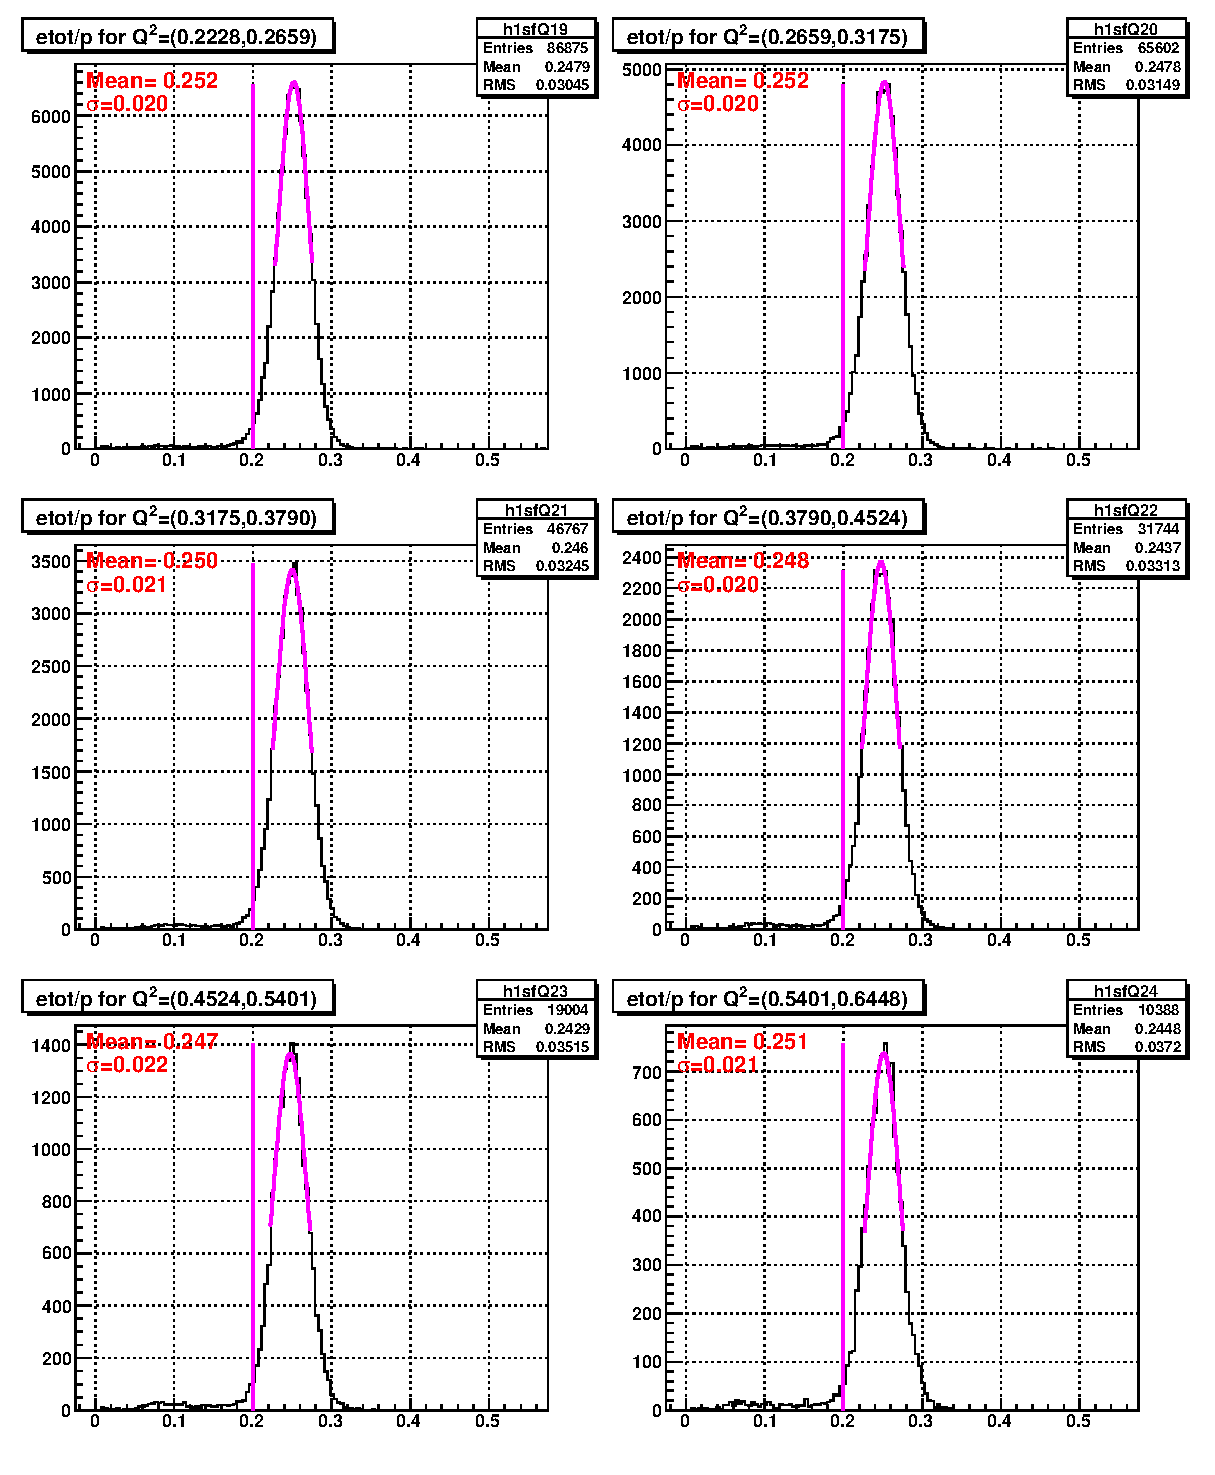
\includegraphics[width=1.0\textwidth]{chap4simul/FigCuts/ecCuts_sfOneD_Eb2_4ThN.eps}  %0.6 is the fraction of the real image width????
\leavevmode 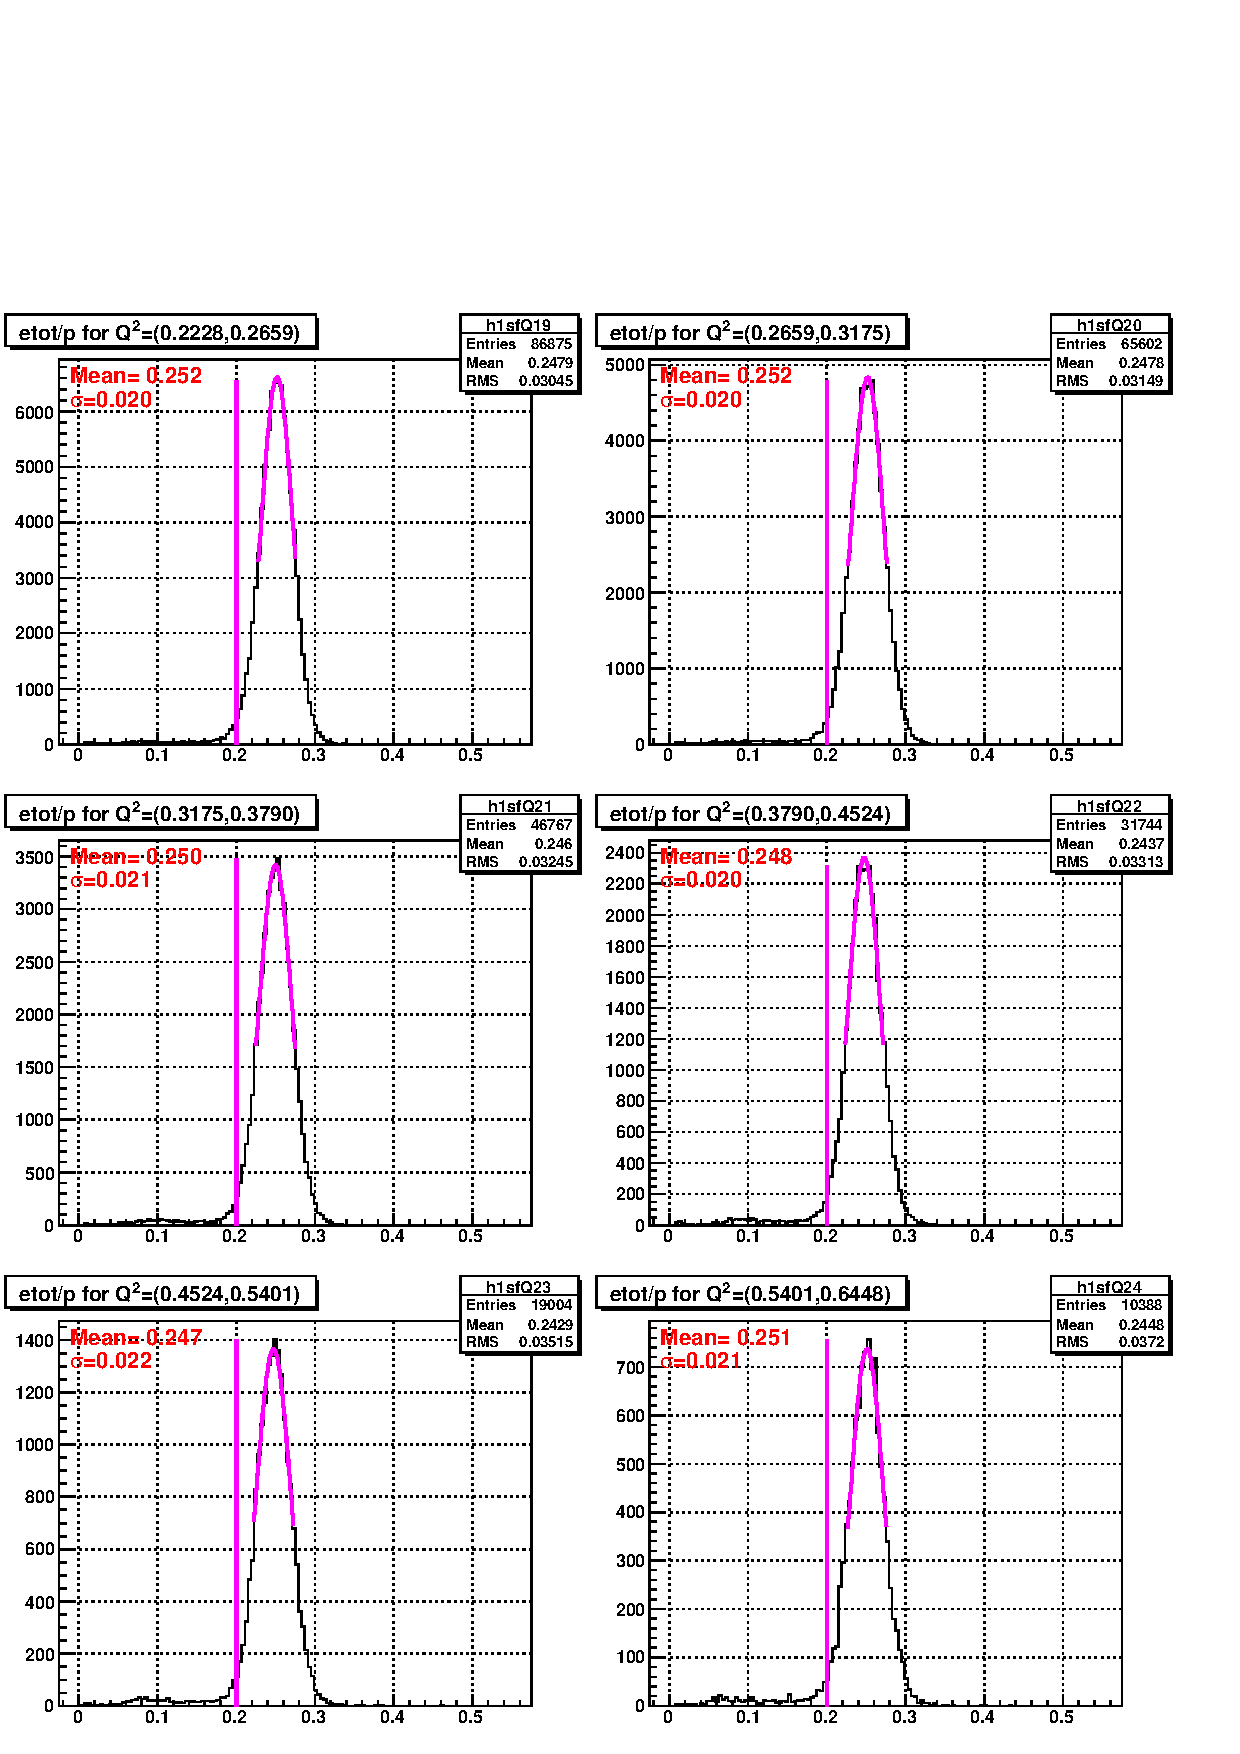
\includegraphics[width=1.0\textwidth]{figuresEG4/FigCuts/ecCuts_sfOneD_Eb2_4ThN.png}  %0.6 is the fraction of the real image width????
\caption[EC sampling fraction cut (Exp.)]{The \qsqs dependent cuts on the EC sampling fraction for 2.0 GeV experimental data. Events below the red lines are rejected.}
\label{ecSfExp6}
\end{figure}



\begin{figure}[H]%[htp] %ht, htpb (p - float, b = bottom, h=? t = top)
\centering
%\leavevmode 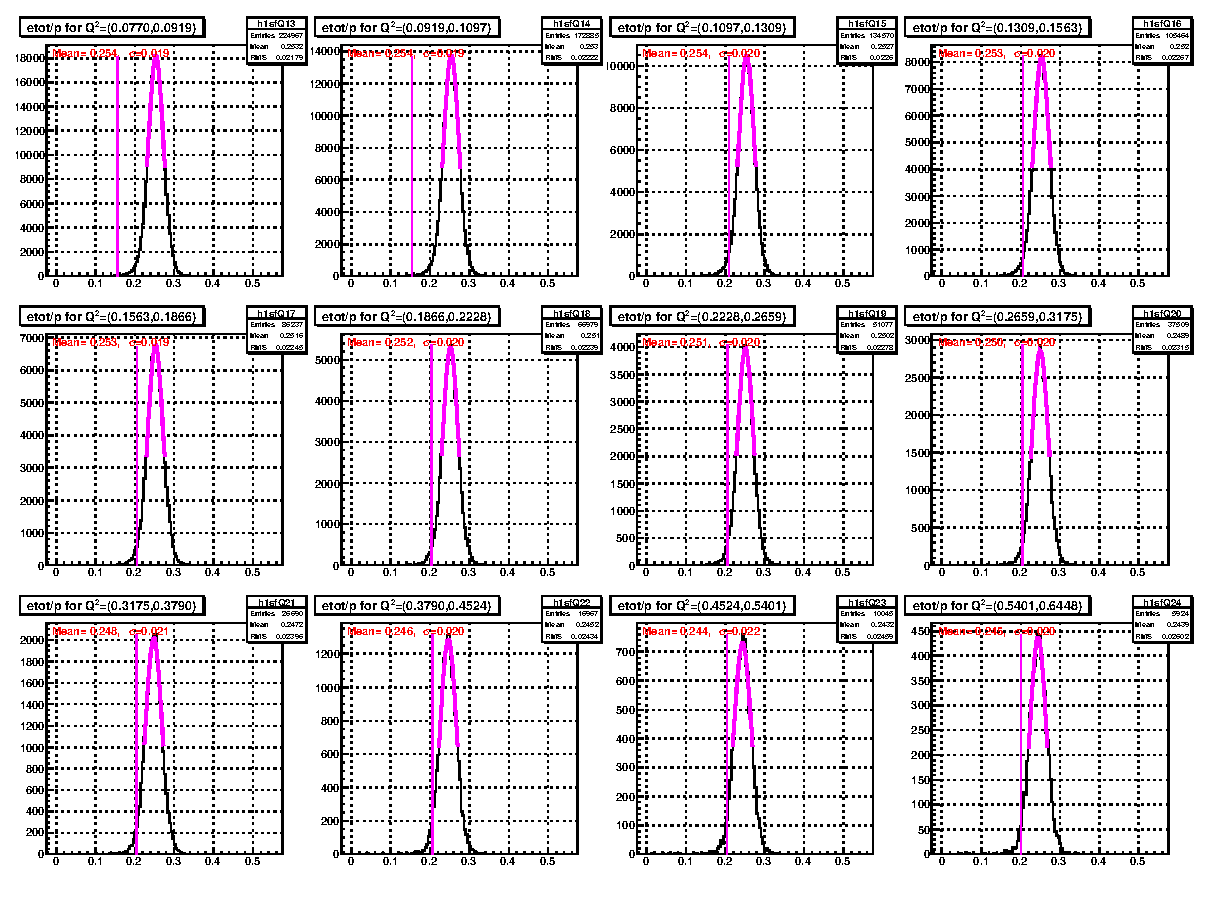
\includegraphics[width=1.0\textwidth]{chap4simul/FigCuts/ecCuts_sfOneD_Eb2_4Thsim.eps}  %0.6 is the fraction of the real image width????
%\leavevmode 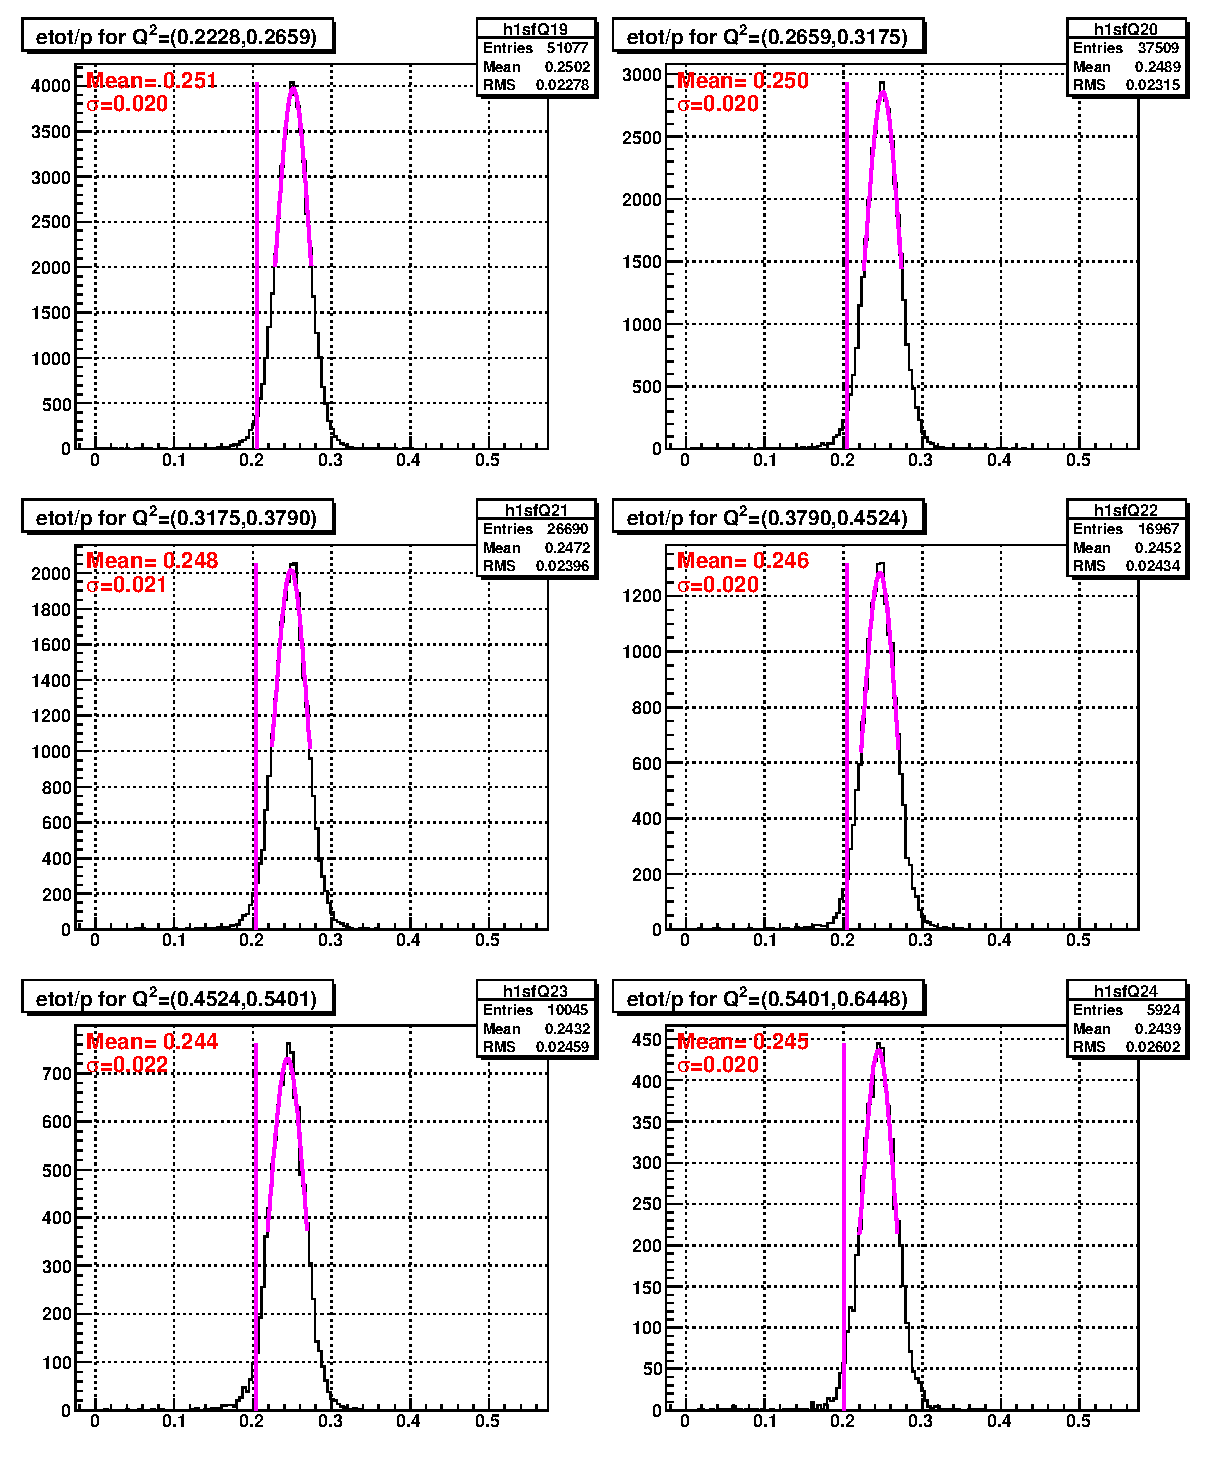
\includegraphics[width=1.0\textwidth]{chap4simul/FigCuts/ecCuts_sfOneD_Eb2_4ThsimN.eps}  %0.6 is the fraction of the real image width????
\leavevmode 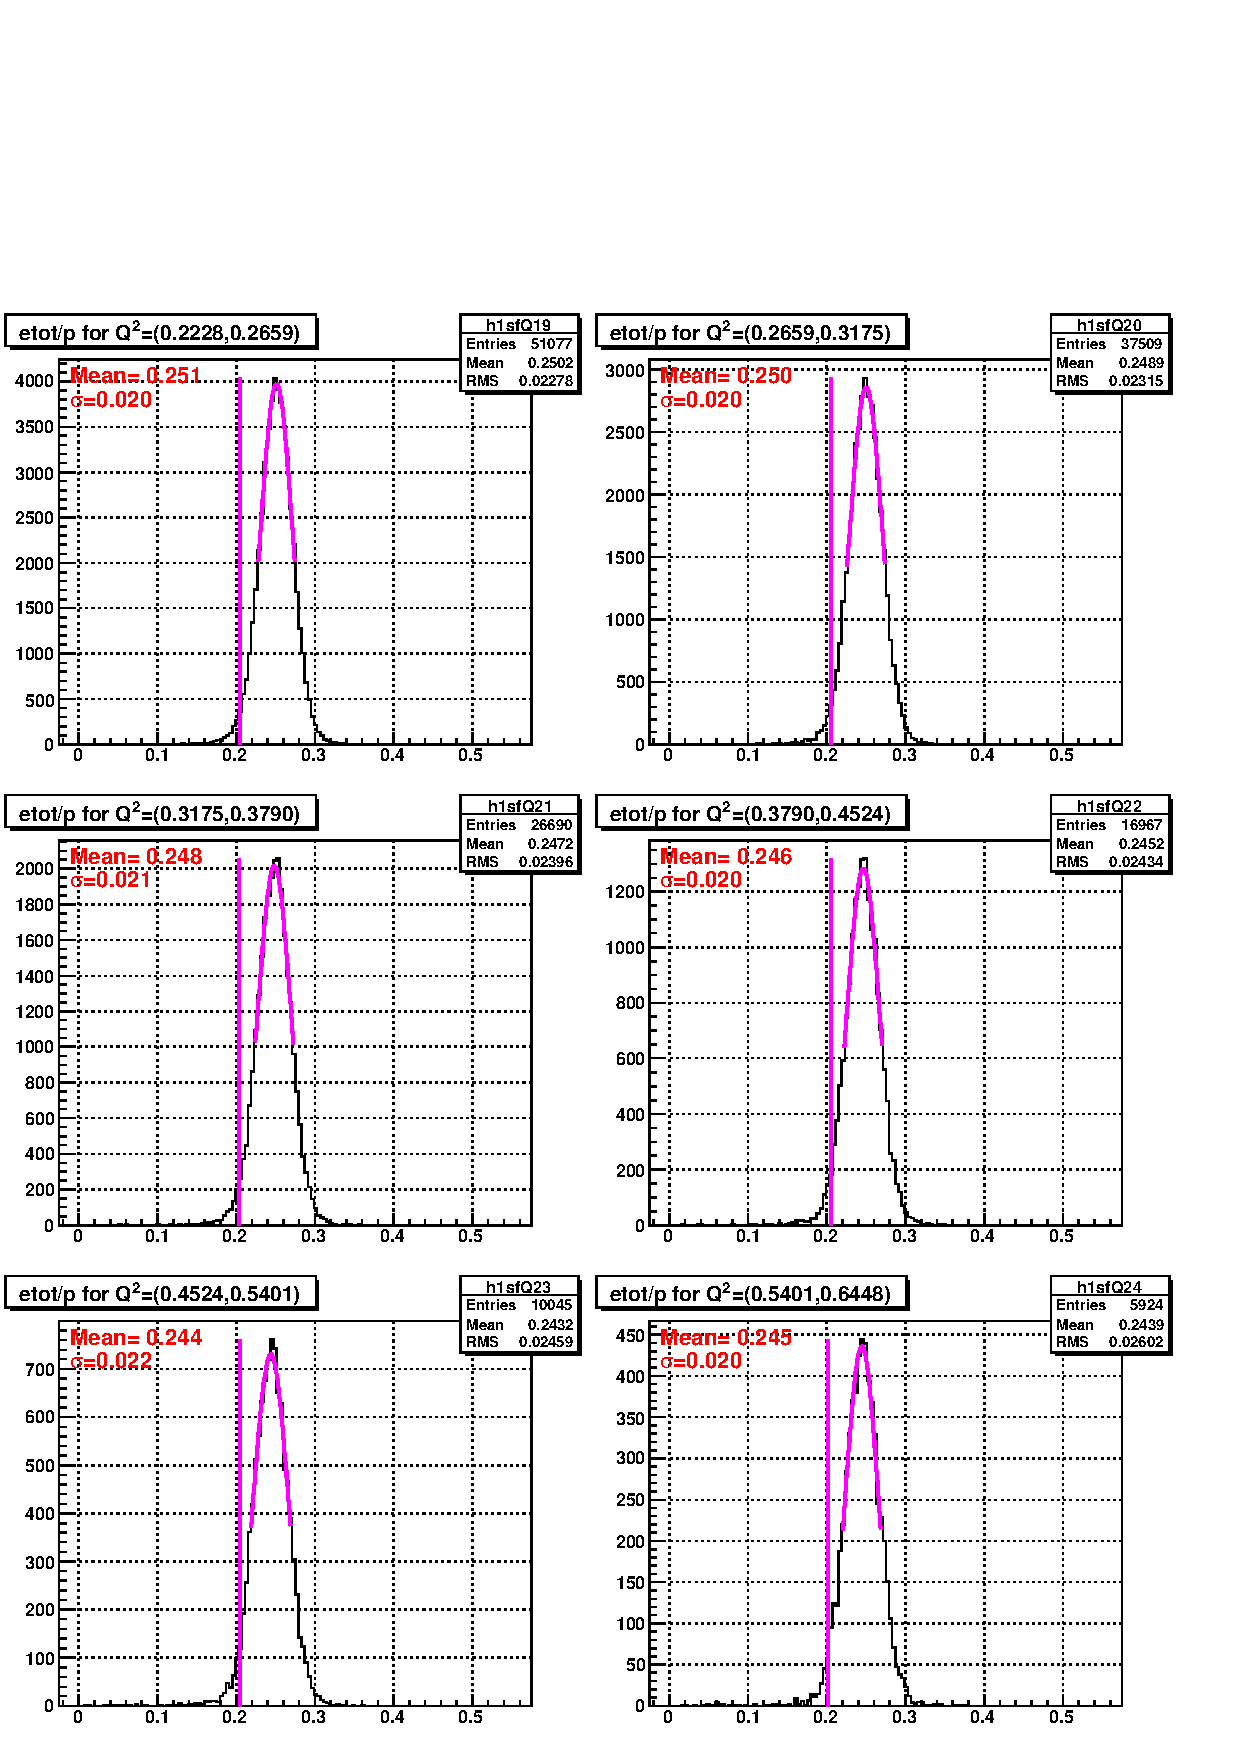
\includegraphics[width=1.0\textwidth]{figuresEG4/FigCuts/ecCuts_sfOneD_Eb2_4ThsimN.png}  %0.6 is the fraction of the real image width????
\caption[EC sampling fraction cut (Sim.)]{The \qsqs dependent cuts on the EC sampling fraction for 2.0 GeV simulation data. Events below the red lines are rejected.}
\label{ecSfSim6}
\end{figure}


%In short, only two numbers 0.15 and 0.2 define the cuts on the experimental data, but the cuts for simulation data are all different, yet they are at the same relative distance from the electron peaks as in the experimental data and, therefore, include about the same fraction of good electrons. 

%\textbf{\textcolor{red}{This section may have been too verbose and complex to understand.}}
% http://en.wikipedia.org/wiki/Particle_shower:   An ``electromagnetic shower'' begins when a high-energy electron, positron or photon enters a material. At high energies (above a few MeV, below which photoelectric effect and Compton scattering are dominant), photons interact with matter primarily via pair production  that is, they convert into an electron-positron pair, interacting with an atomic nucleus or electron in order to conserve momentum. High-energy electrons and positrons primarily emit photons, a process called bremsstrahlung. These two processes (pair production and bremsstrahlung) continues until photons fall below the pair production threshold, and energy losses of electrons other than bremsstrahlung start to dominate. 
%In the case of experimental data, the sampling fraction is cut at 0.2 in the first fourteen \qsqs bins and at 0.15 in the others. But, in the case of simulated data, the cuts are variable, but still are correlated with the cuts on the real data. To ensure the proportional/same fraction of events from both real and simulated data in a given \qsqs bin, the electron peaks on those data are first fitted to Gaussian distributions to find the peak position and width (represented by $\sigma$ i.e. the standard deviation), and then cut position on simulated data is determined by the value which is at the same distance from  the average in terms of $\sigma_{sim}$ as the cut on real data is from its own mean in terms of $\sigma_{exp}$.






\subsubsection{Cuts on $E_{in}$}
\begin{figure}[h] %ht, htpb (p - float, b = bottom, h=? t = top)
\centering
%\leavevmode 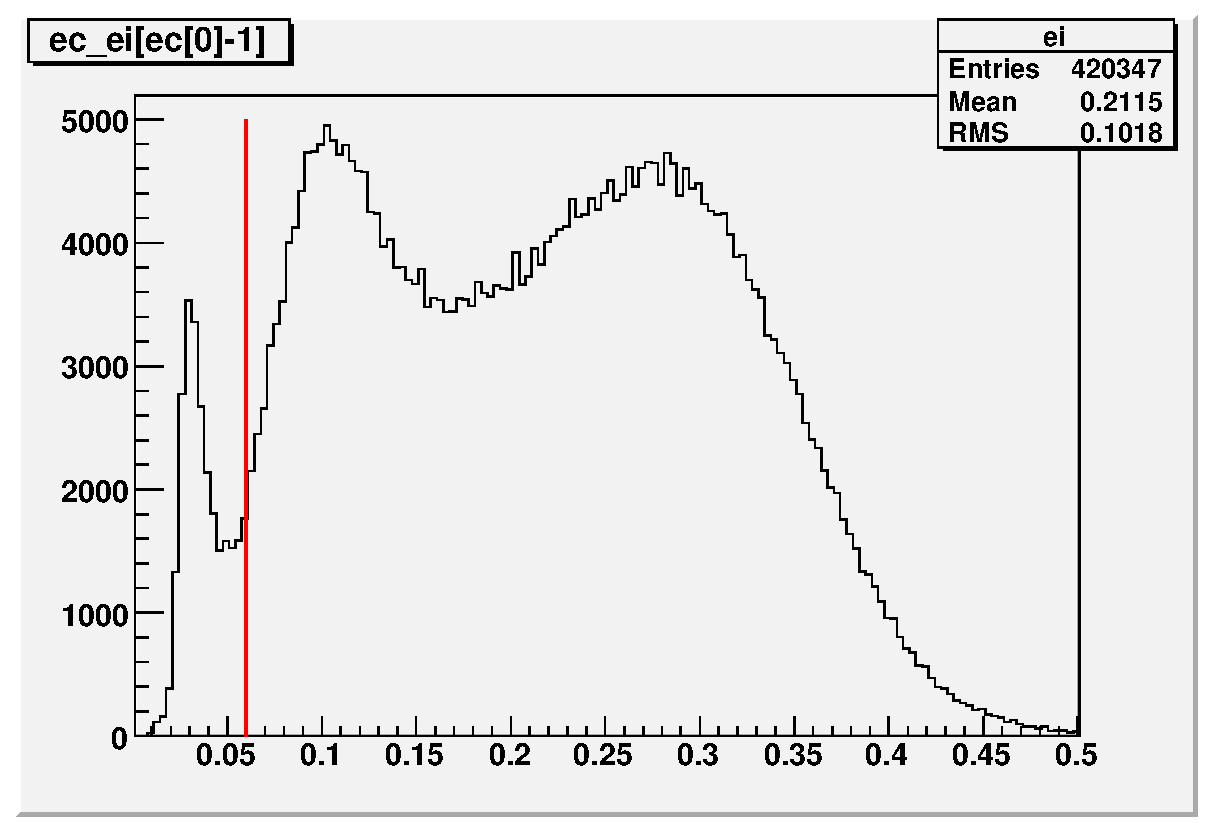
\includegraphics[width=0.8\textwidth]{chap4simul/FigCuts/ec_eiCutFrmRtPrmtClasEb2.eps}  %0.6 is the fraction of the real image width????
\leavevmode 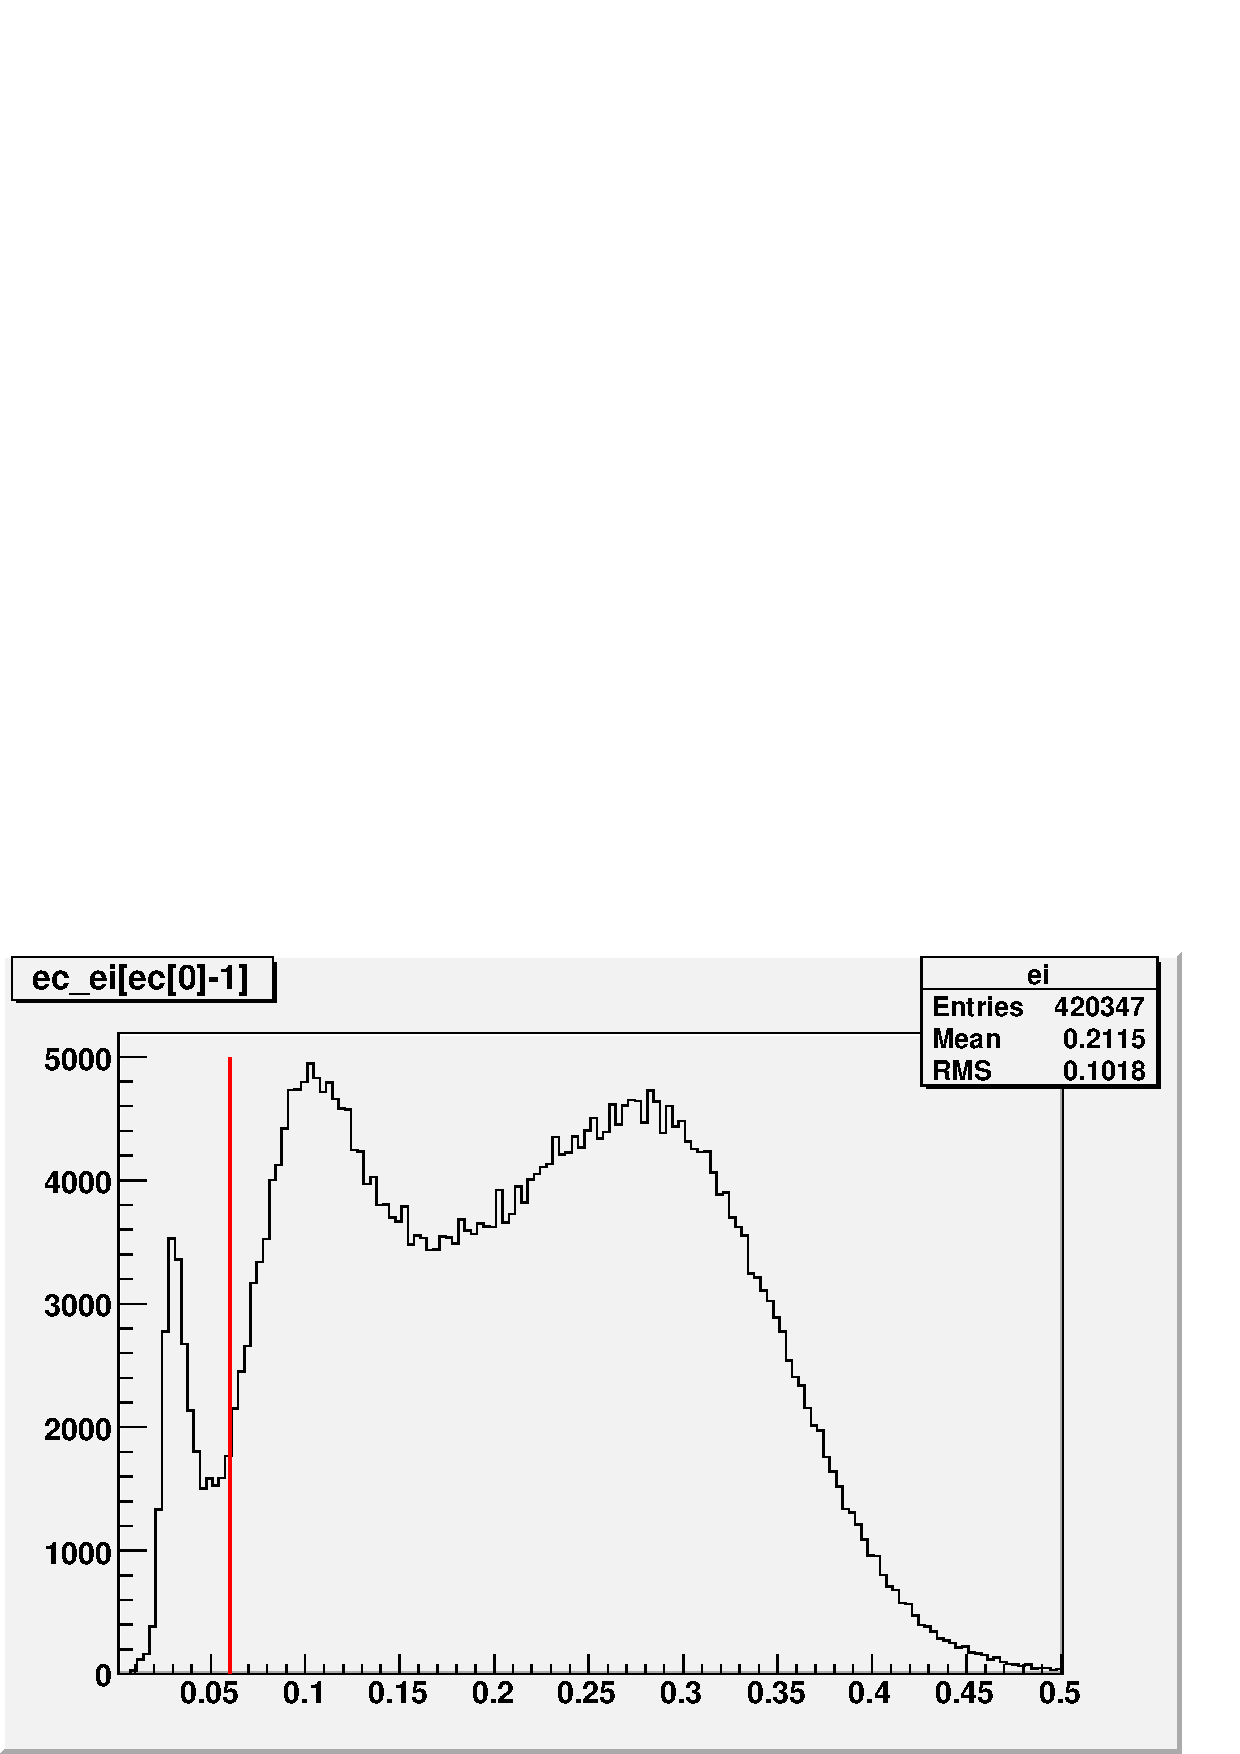
\includegraphics[width=0.8\textwidth]{figuresEG4/FigCuts/ec_eiCutFrmRtPrmtClasEb2.png}  %0.6 is the fraction of the real image width????
\caption[EC inner energy cut (2.0 GeV)]{Energy deposited (GeV) in the inner EC and the cut (red line) used to reject pions (seen as a peak at about 0.03 GeV) from a sample of electron candidates of 2.0 GeV data.}
\label{ecInExp1}
\end{figure}

Pions, which do not shower and are minimum ionizing particles in the momentum range detected in CLAS, deposit only a small amount of energy in the inner part of the EC, %in the ratio of about 5:3, independent on their momentum. %https://userweb.jlab.org/~ungaro/maureepage/proj/pi0/e_pid/note/electron_pid.html#x1-100001.7
independent of their momentum. When $E_{in}$ is histogrammed, the small pion signal peak at about 0.03 clearly stands out from the large electron sample, with little overlap in between. So, a universal cut of $E_{in}$=0.05 on both data and simulation (as shown in Figs. \ref{ecInExp1}, \ref{ecInExp6} and \ref{ecInSim6}) safely rejects most of the pions from the electron candidate sample. 


\begin{figure}[H]%[hp] %ht, htpb (p - float, b = bottom, h=? t = top)
\centering
%\leavevmode 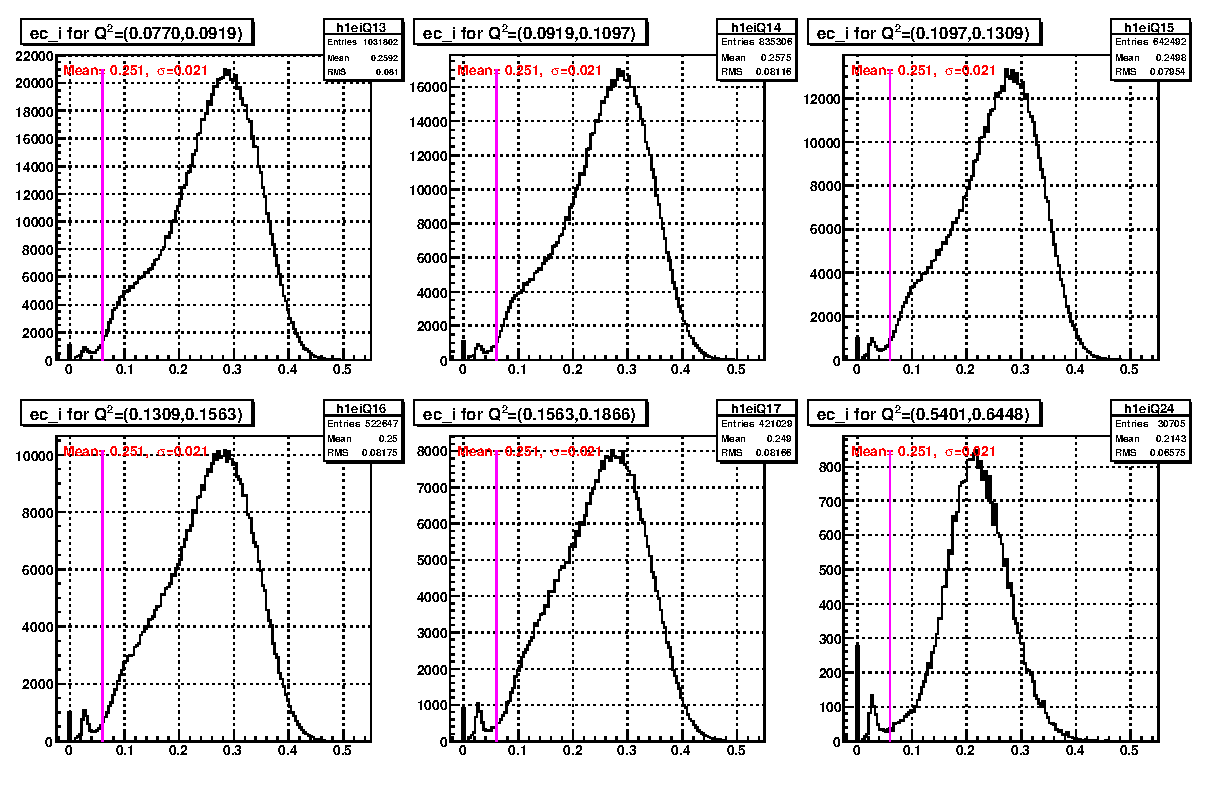
\includegraphics[width=1.0\textwidth]{chap4simul/FigCuts/ecCuts_eiOneD_Eb2_4Th.eps}  %0.6 is the fraction of the real image width????
\leavevmode 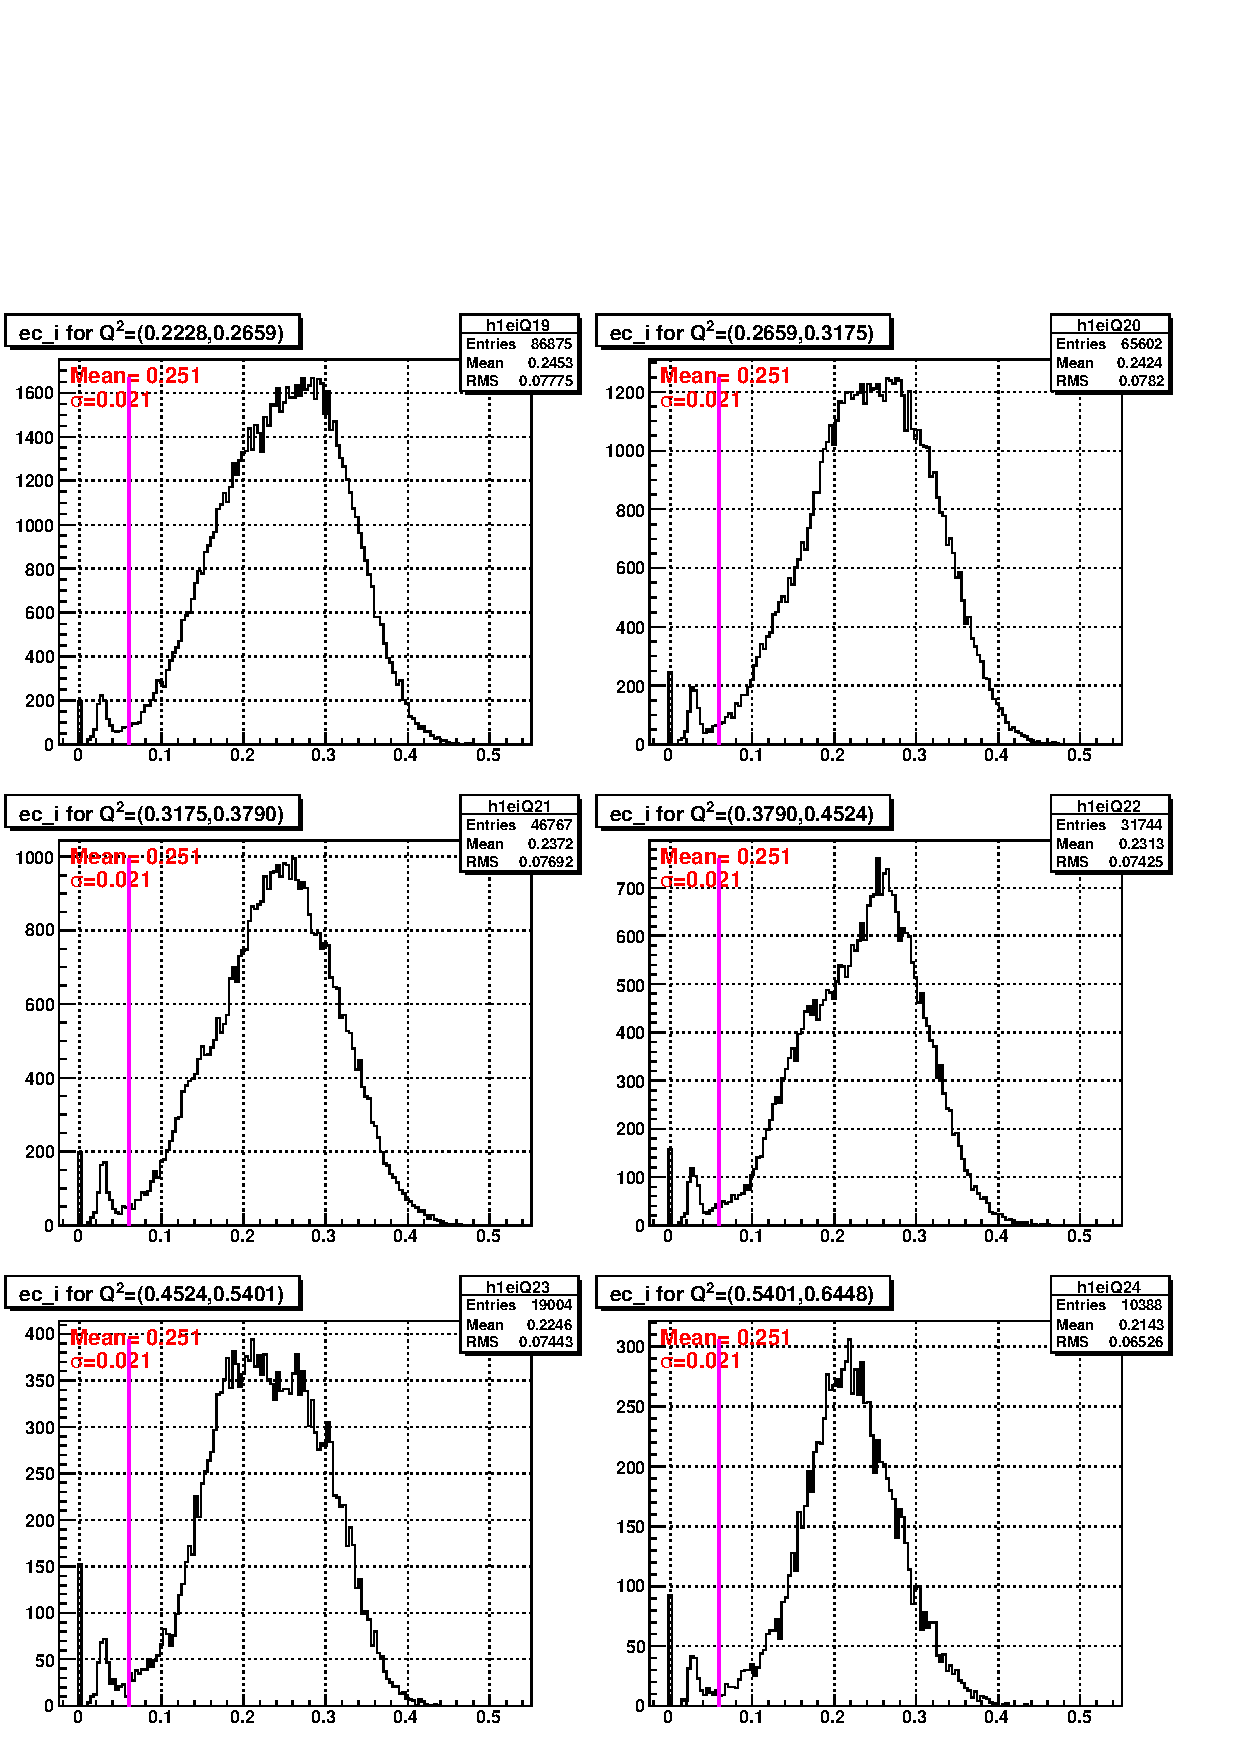
\includegraphics[width=1.0\textwidth]{figuresEG4/FigCuts/ecCuts_eiOneD_Eb2_4ThN.png}  %0.6 is the fraction of the real image width????
\caption[EC inner energy cut (Exp.)]{The EC-inner cut on a sample of 2.0 GeV experimental data in various \qsqs bins.}
\label{ecInExp6}
\end{figure}



\begin{figure}[H]%[hp] %ht, htpb (p - float, b = bottom, h=? t = top)
\centering
\leavevmode 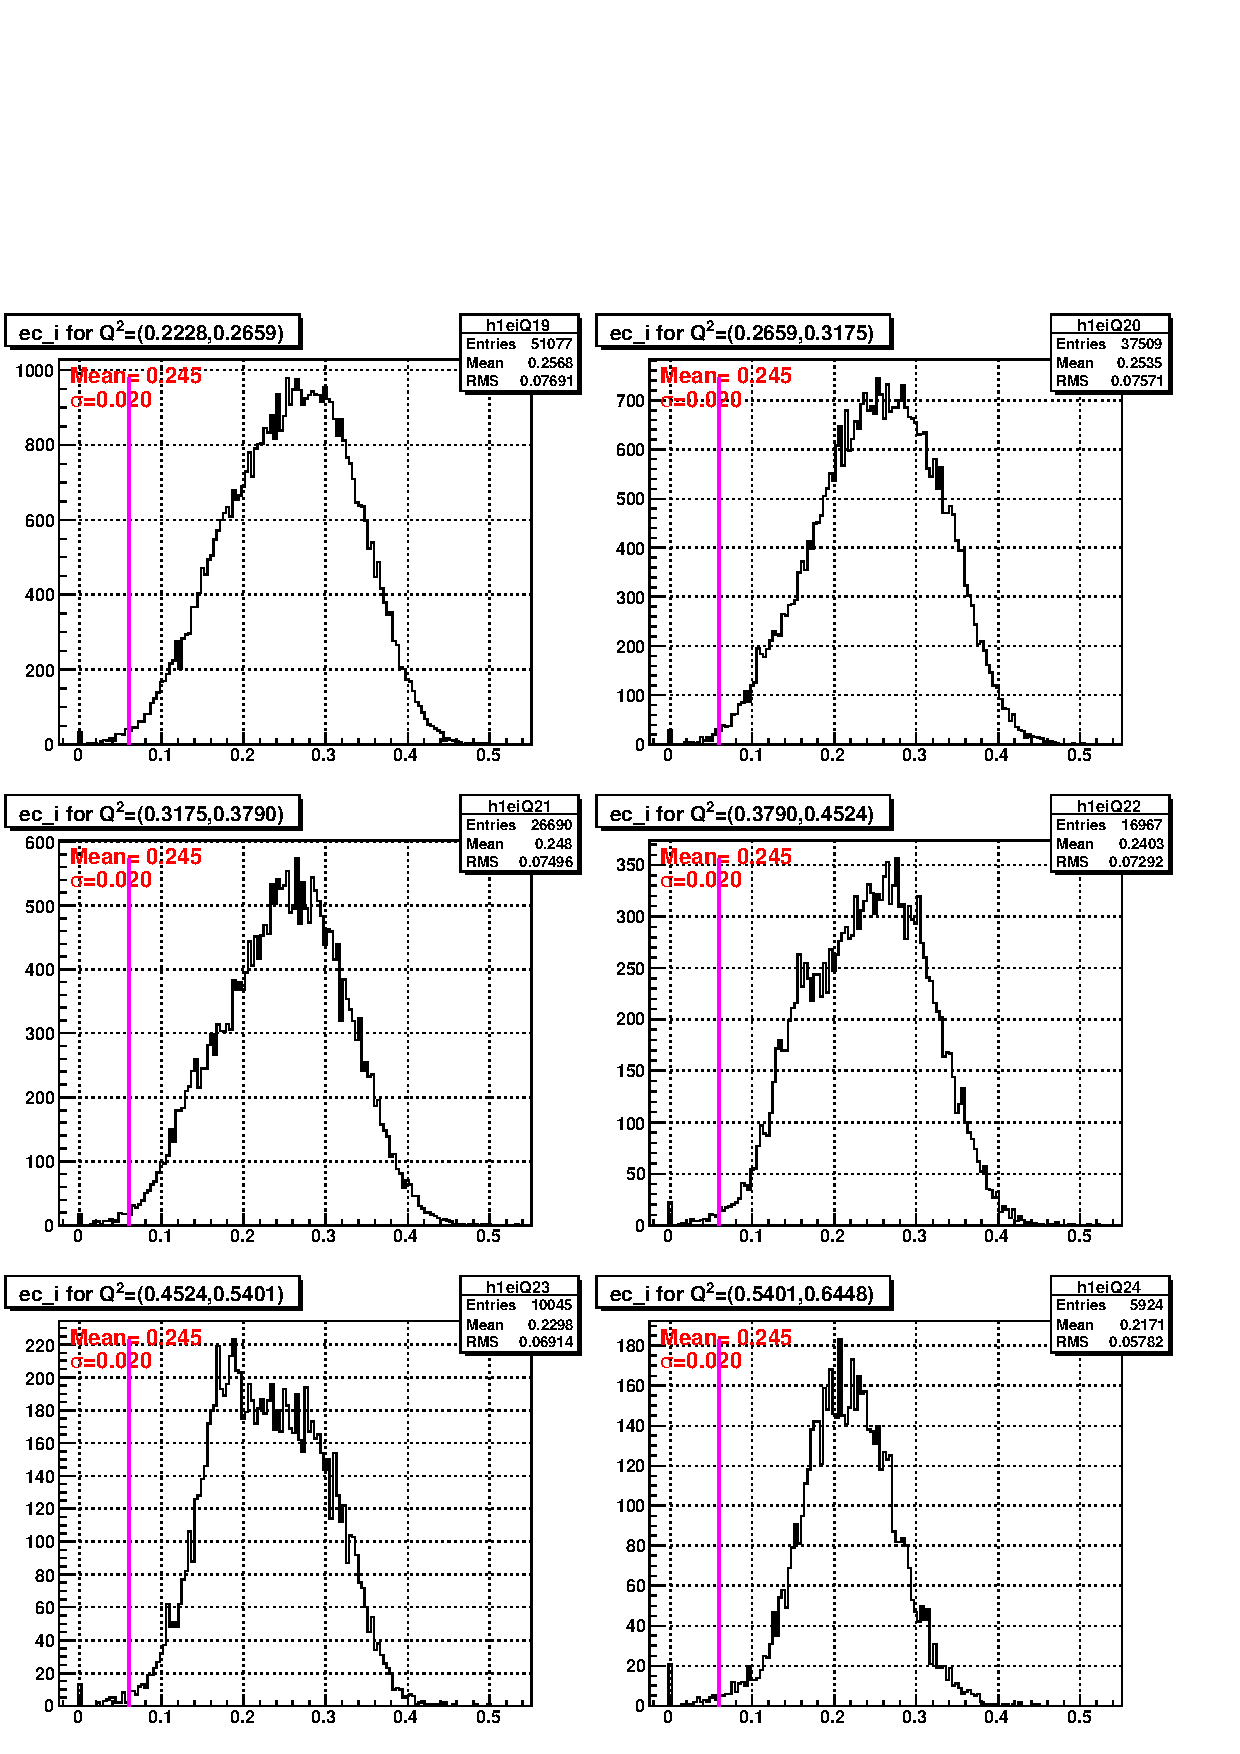
\includegraphics[width=1.0\textwidth]{figuresEG4/FigCuts/ecCuts_eiOneD_Eb2_4ThsimN.png}  %0.6 is the fraction of the real image width????
\caption[EC inner energy cut (Sim.)]{The EC-inner cut on a sample of 2.0 GeV simulation data in various \qsqs bins.}
\label{ecInSim6}
\end{figure}




\begin{comment} %Part copied from my thesis (just to remind myself what I had done)

\subsubsection{Cuts on $E_{out}$}
In addition to the two EC-cuts above, one more cut based on the correlation between EC-outer and EC-inner %ec\_o/p and ec\_i/p 
(as shown in Fig. \ref{ecOvI}) was used which helps further to clean up the electron sample. %pion contamination. %%%SEK cor.

\begin{figure}[H]%[h] %ht, htpb (p - float, b = bottom, h=? t = top)
\centering
\leavevmode 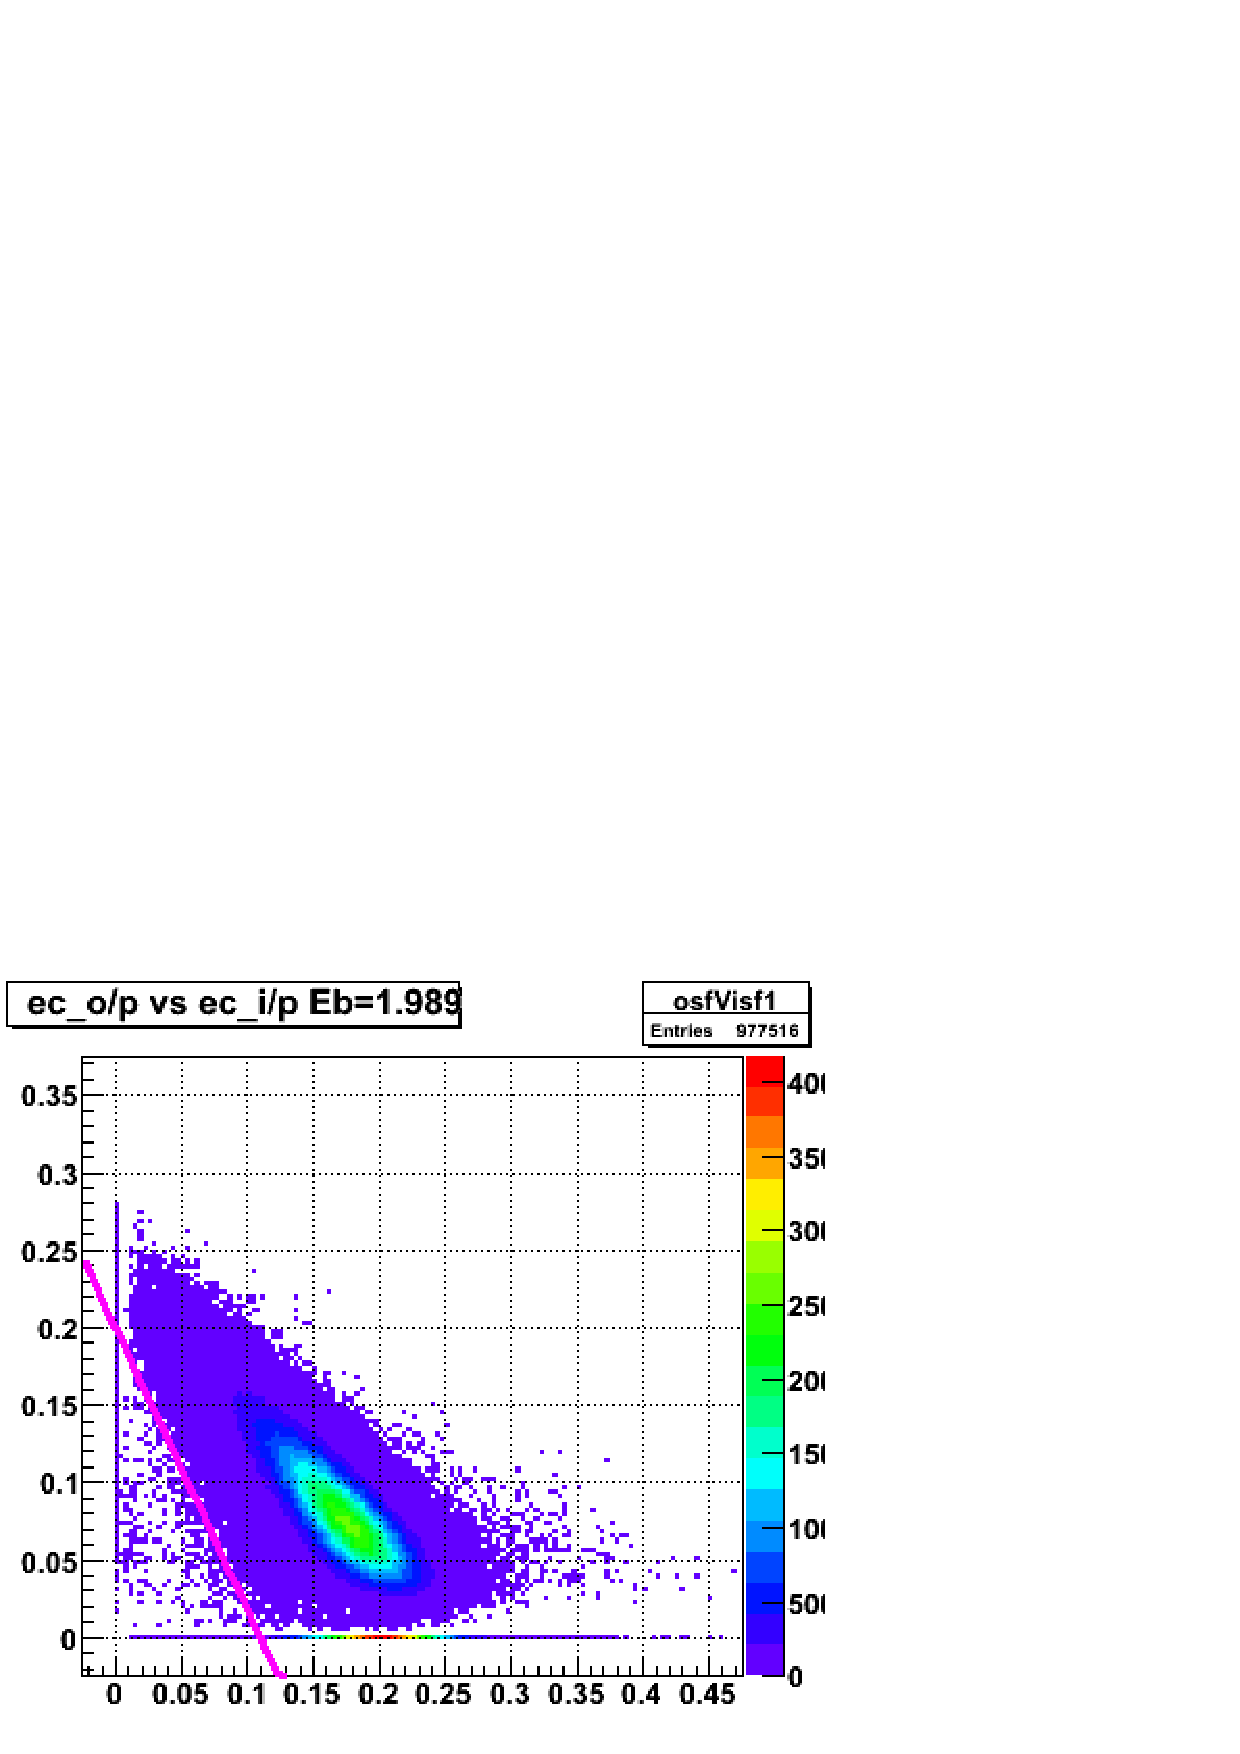
\includegraphics[width=0.8\textwidth]{figuresEG4/FigConv/stdECcutsSfovSfi_Eb2sim.png}  %0.6 is the fraction of the real image width????
\caption[EC inner and outer energy cut (Exp.)]{Energy detected in EC outer as a function of EC inner, both normalized with the particle momentum, for the 2 GeV data. The brown line shows the EC cut to reject pions (which fall below that line).}
\label{ecOvI}
\end{figure}

\end{comment}
